\section{Approach} \label{sec:approach}

We determine a measurement noise
model for the Kinect sensor through statistical analysis of experimental data.
We have designed our model to be compliant with similar models presented in works such  as \cite{Elfes1989} and the well-known
\cite{Thrun:2005:PR:1121596} by Thrun et al. One thing to note is that these
works aim to build a \emph{sensor model} which takes into account four general
types of measurement errors: measurement noise, unexpected objects, failure to
detect objects, and random unexplained noise. In this work we are focus on modeling the
measurement noise component of the sensor model. In \cite{Thrun:2005:PR:1121596} the measurement
noise component is named $p_{hit}$ and formally defined it as: 
%
{
\setlength\abovedisplayskip{7pt} \setlength\belowdisplayskip{2pt}% needed to make spacing more compact
\begin{equation*}
p_{hit}(z_t^k|x_t,m) = \eta \  \left(2\pi\sigma^2_{hit}\right)^{-1/2} \text{exp}\left(-\frac{1}{2}\frac{z_t^k-z_t^{k*}}{\sigma^2_{hit}}\right)
\label{eq:mp} 
\end{equation*}
}
%

\noindent Using this definition, the measurement noise is modeled as a narrow Gaussian centered about $z_t^{k*}$ and with standard deviation of $\sigma_{hit}$. The Probability Density Function (PDF) is normalized by $\eta$ and is limited to the range $0\leq z_t^k\leq z_{max}$ where $z_{max}$ is the maximum sensor range.  The ``ground truth" sensor reading is denoted by $z_t^{k*}$. This value can be found from an environmental map $m$ and the robot pose $x_t$ via ray tracing. The actual sensor reading is denoted by $z_t^k$. The PDF is defined using the difference between the actual sensor reading and the ground truth. Also, $\sigma_{hit}$ is a constant, intrinsic noise parameter which, in practice, is often set by hand. In \cite{Thrun:2005:PR:1121596} a methodology to learn $\sigma_{hit}$ through experimentation is described. 

Our work determines $\sigma_{hit}$ for the Kinect sensor from a large experimental data set. There are two fundamental issues to consider when determining this parameter:  

\begin{itemize}
\item  First, $\sigma_{hit}$ is not simply a constant value. It has been observed \cite{Fallon2012} and \cite{Newcombe2011} that the quality of measurements from the Kinect is dependent on the measurement distance $d$ and also the angle of incidence $\alpha$. Therefore, we modeled $\sigma_{hit}$ as a function $\sigma_{hit}(\alpha,d)$. 
\item Second, when ground truth is determined with an environmental map $m$ and robot pose $x_t$, the data set is not guaranteed to contain a thorough sampling of $\alpha$ and $d$ combinations. Therefore, we developed an economical method to obtain a data set with a thorough sampling. 
\end{itemize}

%\noindent Our solutions for approaching these fundamental issues are what and makes it of value to the robotics community. 
\noindent The solutions that we present for approaching these fundamental issues is what sets our work apart and makes it of value to the robotics community. 

The remainder of this section is divided into three subsections. First, in the Data Acquisition subsection, we outline our technique for acquiring our data set. Next, in the Theoretical Discussion subsection, we will have a detailed look at some of the crucial aspects of our method. Finally, will be the Implementation subsection where we will explain the pseudocode of the procedure we used for producing $\sigma_{hit}$ as a function of $\alpha$ and $d$.

\subsection{Data Acquisition} % ______________________________________________________________________

Our data set was obtained by viewing a large flat wall from several different
sensor \emph{poses} with the Kinect. For each \emph{pose}, 30 point cloud
\emph{shots} were acquired. Each point cloud consists of a set of 3D coordinates such that $p=\langle x,y,z \rangle \in \mathbb{R}^3$. Figure \ref{fig:exp_setup} illustrates the data acquisition process. Each \emph{pose}
can be expressed by $(L,\theta)$. Since our method is based on the error of each point $p$ to the wall and the position of the wall is estimated with the point cloud, we do not require accurate positioning of the sensor for each \emph{pose}. The chosen \emph{poses} can be described by the sets 

{\small \setlength\abovedisplayskip{-4pt} \setlength\belowdisplayskip{6pt} % needed to make spacing more compact
\begin{equation*}
\{1,1.5,\dots,5\text{m}\}\times\{0,15,\dots,75\text{\textdegree}\} \cup \{5.5,6,\dots,10\text{m}\}\times\{0,15\text{\textdegree}\}.
\end{equation*}
}%

\noindent We took data from 74 different \emph{poses} such that the distribution of points in the $(\alpha,d)$ space covers most of the region defined by $\{\alpha \in [0^\circ, 90^\circ], \; d \in [0\text{m}, 10\text{m}] \}$.

We also obtained a validation data set using a second Kinect sensor and a ASUS Xtion PRO. For each sensor we chose 4 \emph{poses} which can be described by $\{2.25,3.75m\}\times\{22.5,52.5\text{\textdegree}\}$. These \emph{poses} were chosen to be well spaced in the set of \emph{poses} from our large data set.  

\begin{figure}[h]
\centering
%\subfigure{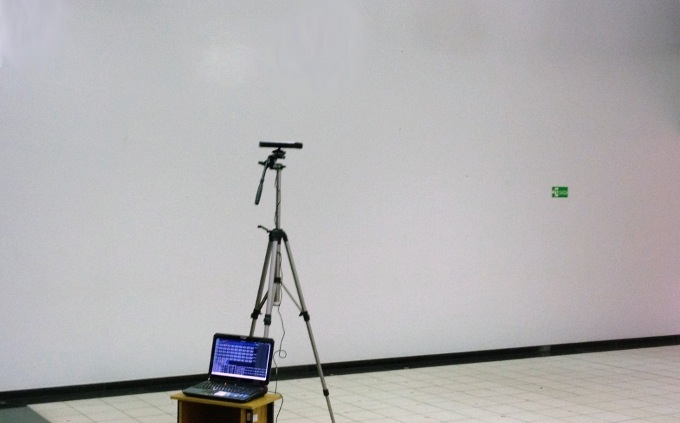
\includegraphics[width=.4\textwidth]{img/expSetup.jpg}} \qquad
%\subfigure{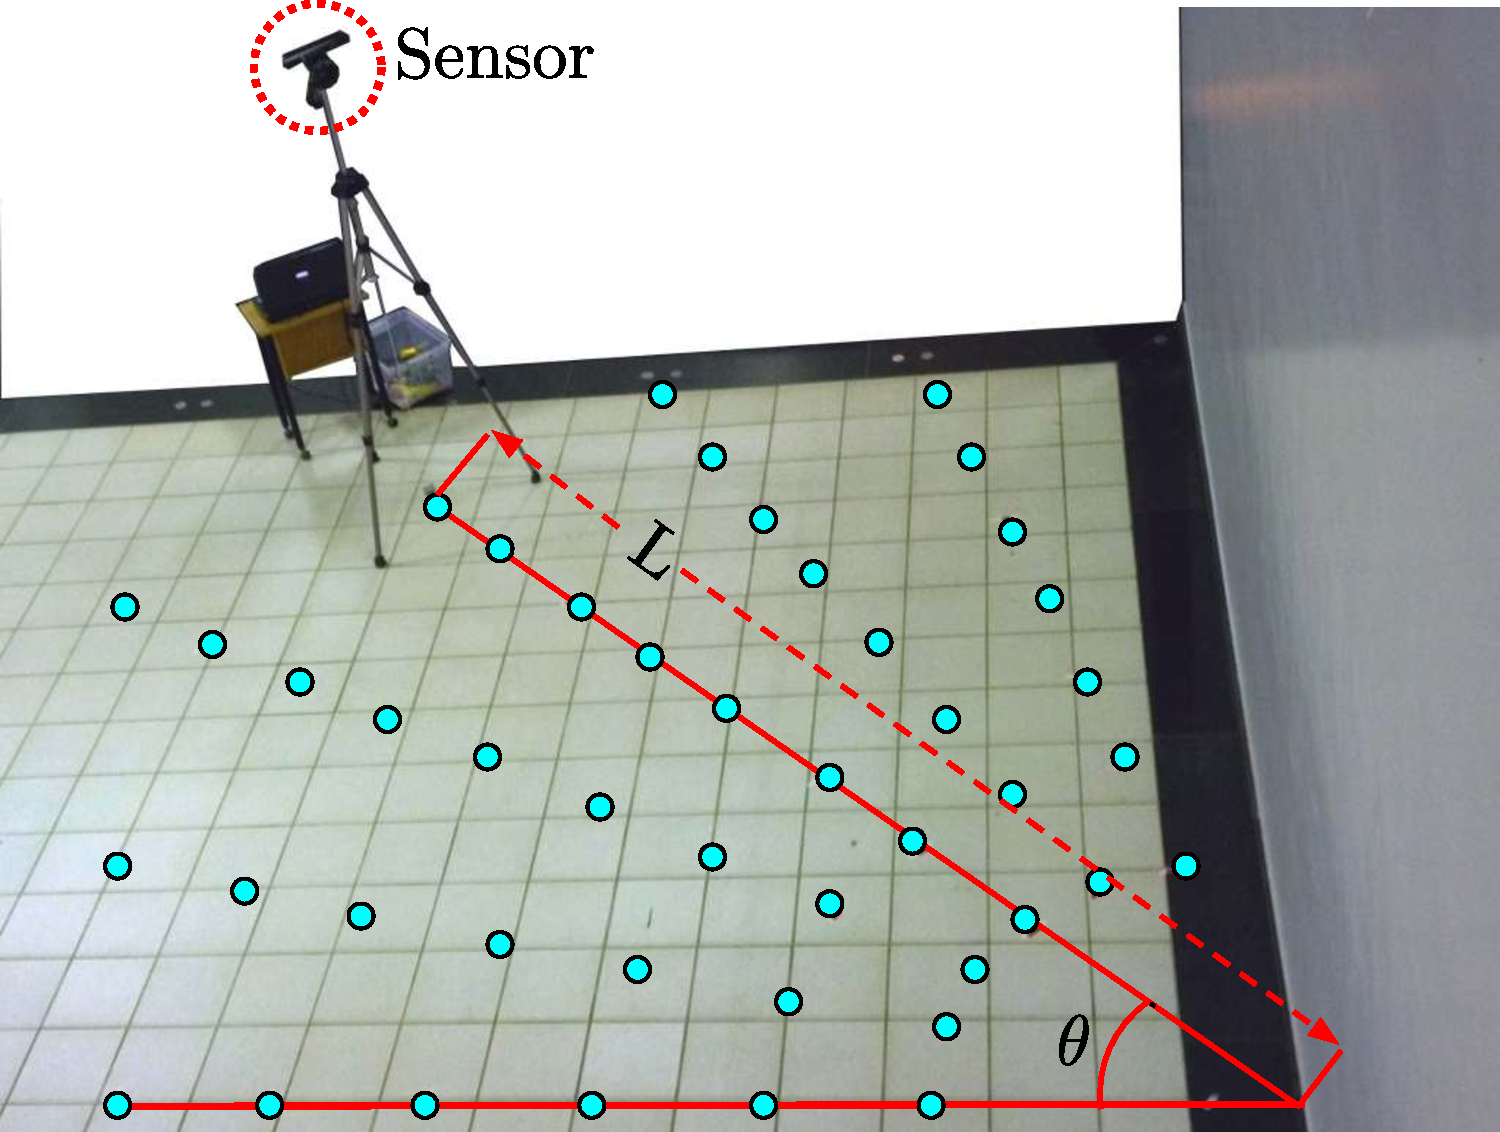
\includegraphics[width=.4\textwidth]{img/expSetup_markers.pdf}} \qquad
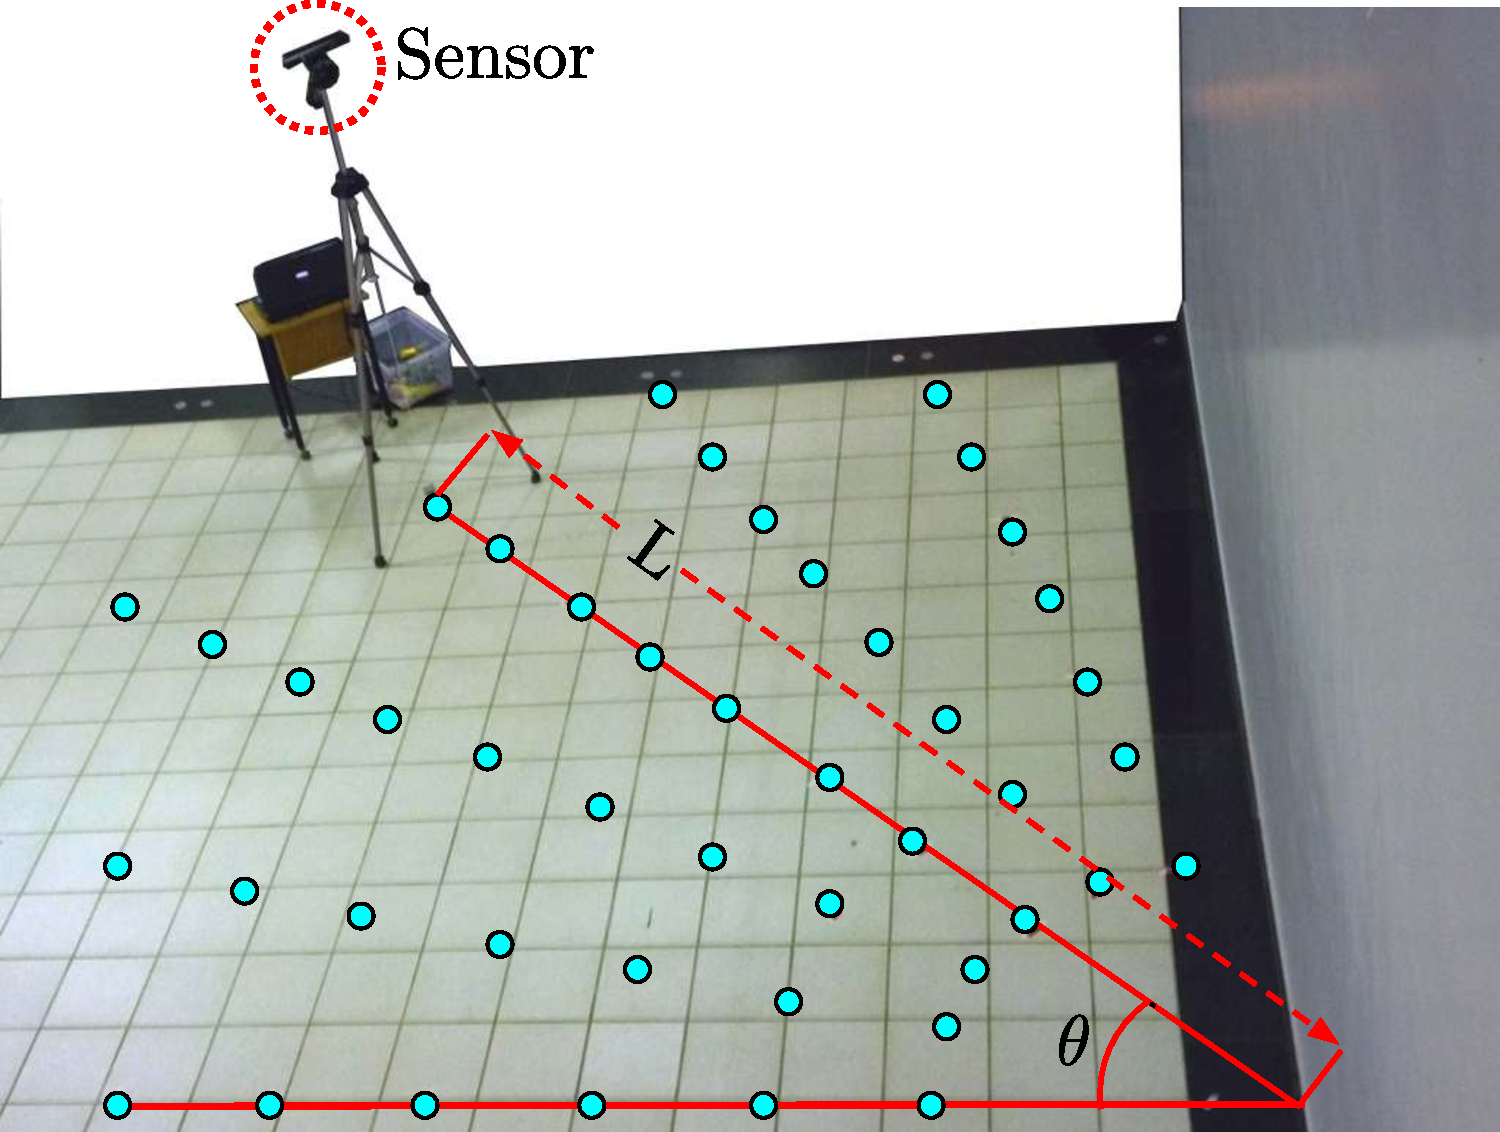
\includegraphics[width=.4\textwidth]{img/expSetup_markers.pdf}
\caption{
Our experimental set-up. The Kinect is viewing the wall from a particular sensor \emph{pose} defined by $(L,\theta)$. The spatial distribution of sensor \emph{poses} for a subset of all \emph{poses} are marked with cyan dots.
}
\label{fig:exp_setup}
\end{figure} 

Special care was taken during the data acquisition process in order to obtain our data set. We made sure that environmental factors such as lighting and temperature were typical of an office environment and did not vary significantly. Also, we post processed the data in order to remove small portions of point clouds which were not measurements of the wall, such as the floor. Finally, the 30 \emph{shots} acquired at each \emph{pose} were captured with the sensor completely still.

\subsection{Theoretical Discussion} 

Let us investigate some of the crucial theoretical aspects of our methodology before moving on. To begin, we will define an initial framework of our data acquisition process. First let us define the indices used in our framework: $a$ is an index of all points in a single point cloud, $b$ is an index of all \emph{shots} for a single \emph{pose}, and $c$ is the index of all \emph{poses}, such that:

{\setlength\abovedisplayskip{-4pt} \setlength\belowdisplayskip{-4pt} % needed to make spacing more compact
\begin{gather*}
a \in \{1,2,\dots,n_a\};\ b \in \{1,2,\dots,n_b\};\ c \in \{1,2,\dots,n_c\}.
\end{gather*}
} 

\noindent We will now define our estimate of the ``ground truth''. For each \emph{pose} we define a wall by finding the best fit plane of all \emph{shots} from that particular \emph{pose}. The wall is defined by a point on the plane $\overline{p}_c$ and a unitary directional vector $n_c$ by $W_c = [n_c, \overline{p}_c]$, where $\overline{p}_c$ is the centroid of all the \emph{shots}
{
\setlength\abovedisplayskip{4pt} \setlength\belowdisplayskip{2pt} % needed to make spacing more compact
\begin{equation} 
\overline{p}_c=\frac{1}{n_an_b}\sum_{b=1}^{n_b}\sum_{a=1}^{n_b}p_{ab}  
\end{equation}
}

\noindent and $n_c$ is the normal of the best fit plane found by using the centroid value and running a Principal Component Analysis (PCA) analysis for all points. 

Let $i\in\{1,2,\dots,n_an_bn_c\}$ index all points from the entire data set. Then given a point $p_i$, we define the projected point $p_i'$, incident angle $\alpha_i$, distance $d_i$, and error $e_i$. 

{
\setlength\abovedisplayskip{-5pt} \setlength\belowdisplayskip{-4pt} % needed to make spacing more compact
\begin{align}
e_i & = (p_i-\overline{p}_c)\cdotp n_c \label{eq:X1}, \\ 
p_i' &= p_i-n_ce_i \label{eq:X2}, \\
\alpha_i & =\cos^{-1}\left(\frac{-p_i'}{\|p_i'\|_2}\cdotp n_c\right) \label{eq:X3}, \\
d_i & =\|p_i'\|_2 \label{eq:X4} .
\end{align}
}

\noindent % TODO: This doesn't make sense: For each point, the values $n_c$ and $\overline{p}_c$ are chosen from the wall $W_c$ which the point $p_i$ measured.
It is important to remember that, for each pose, the estimate of the wall is obtained from 30 point cloud \emph{shots} and that this estimate uses points with a large range of $\alpha$ and $d$ values. 

Figure \ref{fig:exp_diagram} illustrates the quantities we have calculated for
each point. Using  (\ref{eq:X1}-\ref{eq:X4}) the points can be represented in a new space
described by $\alpha$ and $d$, which we will denote $X$. The space is defined
such that $x_i \in X \ \forall i$ where $x_i=\langle \alpha_i,d_i\rangle \in \mathbb{R}^2$.
The transformation of the points into this new space $X$ is a central aspect of
our methodology. After this transformation, each point still has an associated
error $e_i$. It is important to remember, the fundamental assumption we have behind
our analysis is that the variance of $e_i$ values is dependent on $\alpha$ and
$d$, so this new representation in $X$ space will allow us to characterize this
dependency. 

\begin{figure}[t]
\centering
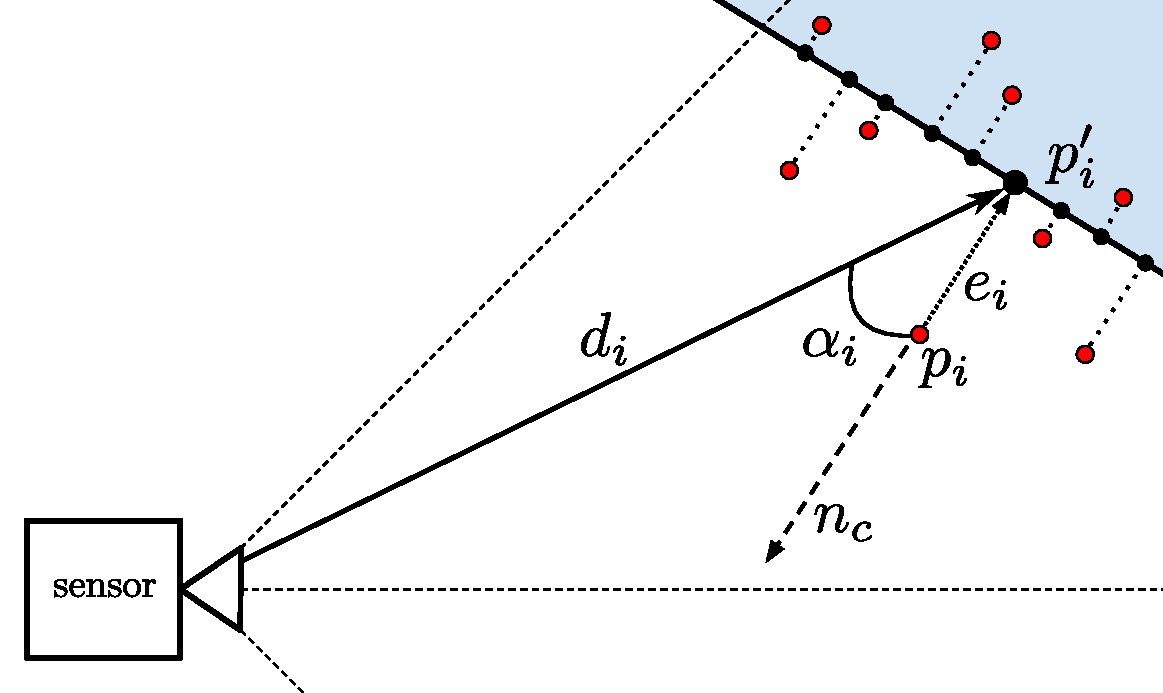
\includegraphics[width=.45\textwidth]{img/ExpDiagram.pdf}
\caption{Diagram showing quantities calculated for each point $p_i$. The blue shaded area represents our estimate of the wall. Red dots represents points from the point cloud. Here we see for a particular point $p_i$, which has measured the wall $W_c$ with normal $n_c$, we can calculate $p_i'$, $\alpha_i$, $d_i$, and $e_i$.}
\label{fig:exp_diagram}
\end{figure} 

In order to have a systematic way to characterize the dependance of the variance of $e_i$ in the space $X$, we have defined a large set of neighborhoods $N_j$ which has an index $j\in [1,2,\dots,n_j]$ where $n_j$ is the number of total neighborhoods. Each neighborhood $N_j$ contains a set of points which have similar $\alpha$ and $d$ values. We define a grid of locations $h_j \in X$ which are the centers of $N_j$. Then each $N_j$ is defined as

{\setlength\abovedisplayskip{-4pt} \setlength\belowdisplayskip{-2pt} % needed to make spacing more compact
\begin{equation}
N_j(h_j,r)  \stackrel{\text{\tiny def}}{=} \{x_i\in X\ \mid \ \|(x_i-h_j)\circ (1,s)\| \leq r\} \\
\end{equation}
}

\noindent where $r$ is the radius of each $N_j$. By adjusting $r$, we are
adjusting the size of the $N_j$ in the $X$ space which lets us control the
similarity of the points in $N_j$. We can also control the scaling on the $d$
axis with $s$. The effect of $s$ can be thought of as a transformation that scales an ellipse $N_j$ into a circle. 
In Figure \ref{fig:spaceCircles} we can visualize a small group of neighborhoods in
the $X$ space. The figure allows us to see how a set of points are grouped
into a single neighborhood. Also, we can see the values we chose for the
spacing between the neighborhoods and the values for defining the radius and scaling. Using this
spacing, $h_j$ becomes a $61\times81 $ grid of points and $n_j=4,941$. 

\begin{figure}[t]
\centering
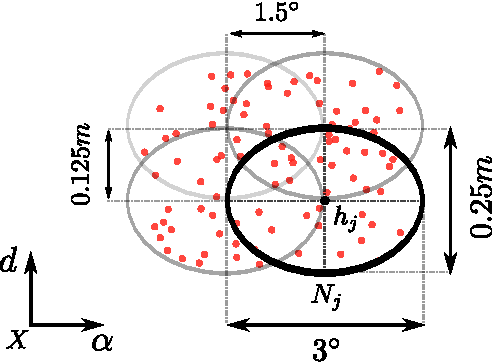
\includegraphics[width=.3\textwidth]{pdfFigs/spaceCircles.pdf}
\caption{Visualization of a small set of neighborhoods $N_j$ and points $x_i$ (colored in red) in the $X$ space. We can see a particular $N_j$ with center $h_j$. $N_j$ is defined by all points within its perimeter.}
\label{fig:spaceCircles}
\end{figure} 

We can now calculate the standard deviation of the error values $e_i$ of the points in each $N_j$ by using the standard deviation equation of (\ref{eq:std}) with $\mu$ defined as the mean. 

{\setlength\abovedisplayshortskip{-2pt} \setlength\belowdisplayshortskip{2pt} % needed to make spacing more compact
\begin{equation}
\sigma_j = \sqrt{ \frac{1}{n_k}\ \sum_{k=1}^{n_k} (e_k-\mu)^2 } 
\label{eq:std}
\end{equation} 
}

\noindent Here $k \in [1,2,\dots,n_k]$ is an index of all points contained within $N_j$. If an $N_j$ has a $k<500$, we do not consider it as part of our model generation. 

% One important note, in our calculations of $\sigma_j$ we use $\mu=0$. Here we will give our reasoning for using an average of zero instead of the sample mean $\overline{e_k}$. Given that the position of the wall $W_c$ is determined by the centroid $\overline{p_c}$, it can be shown that distribution of all $e_i$ will be centered around 0. Figure \ref{fig:distancesToPlane} from our results section shows this with our actual data set. We can then think of the errors of points in each $N_j$ as being samples from a Gaussian processes with known mean by $[e_1,e_2,\dots,e_k ] \sim \mathcal{N}(0,\sigma_2)$. We are interested in finding the best estimate of the sample variance $\hat{\sigma^2}$ so let us define to estimators of  $\hat{\sigma^2}$ as

In our calculations of $\sigma_j$ we assume that the errors are drawn from a
Gaussian process by $[e_1,e_2,\dots,e_k ] \sim \mathcal{N}(\mu,\sigma^2)$. Our
goal is to obtain an estimate of the variance for the samples which we will
denote $\hat{\sigma}^2$. Given that the position of the wall $W_c$ is
determined by the centroid $\overline{p}_c$, it can be shown that the distribution
of all $e_i$ will be centered around 0, i.e. for all points $\mu=0$. For the
sake of simplicity, we assume that this is also the behavior for each
individual neighborhood $N_j$, assigning $\mu_j=0$ to them. Below we further
explain our reasoning behind this assumption. 

We are interested in finding the best estimate of the sample variance $\hat{\sigma}^2$, so let us define the estimators of $\hat{\sigma}^2$ as

%Given that the position of the wall $W_c$ is determined by the centroid $\overline{p_c}$, it can be shown that distribution of all $e_i$ will be centered around 0. Figure \ref{fig:distancesToPlane} from our results section shows this with our actual data set. We can then think of the errors of points in each $N_j$ as being samples from a Gaussian processes with known mean by $[e_1,e_2,\dots,e_k ] \sim \mathcal{N}(0,\sigma_2)$. We are interested in finding the best estimate of the sample variance $\hat{\sigma^2}$ so let us define to estimators of  $\hat{\sigma^2}$ as

{
\setlength\abovedisplayskip{-2pt} \setlength\belowdisplayskip{2pt} % needed to make spacing more compact
\begin{align}
T_1 &= \frac{1}{n_k}\sum_k(e_k-0)^2 \\
T_2 &= \frac{1}{n_k-1}\sum_k(e_k-\overline{e}_k)^2 \ .
\end{align}
}

\noindent We can then compare these estimators by calculating the ratio of the mean squared error (MSE).  

\begin{multline}
\frac{MSE_1}{MSE_2} = \frac{E(T_1-\sigma^2)}{E(T_2-\sigma^2)} = \frac{bias(T_1)+Var(T_1)}{bias(T_2)+Var(T_2)} \\ = \frac{ \frac{\sigma^4Var(\chi_k^2)}{k^2} } { \frac{\sigma^4Var(\chi_{k-1}^2)}{(k-1)^2} } = \frac{k-1}{k} < 1.
\end{multline}

\noindent From the ratio of the MSE values we can say that setting $\mu_j = 0$
gives a better estimate of $\sigma_j$. In addition, we have calculated
$\overline{e}_k$ for each $N_j$, as can be seen in Figure
\ref{fig:sampleMeanFigure}. Since the overall mean values are distributed close
to zero, we are confident that the zero mean assumption does not compromise the
quality of our model, while giving us the benefits of a simpler model. 

\subsection{Implementation} 

Our method is summarized in Algorithm \ref{alg:NS}. It takes about 6 hours to process our complete dataset with a MatLab code, and about 2 hours to process it with the equivalent C++ version. Our code is freely available in a public repository\footnote{More info about the repository can be reached through http://www.verlab.dcc.ufmg.br/projetos/kinect-measurement-noise-model}.

\algsetup{indent=1em}
\begin{algorithm}[htpb]
\caption{$\ \ \sigma(\alpha,d)=GenerateModel(p_{abc})$} 
\label{alg:NS}
\begin{algorithmic}%[1]
\vspace{1mm}
\STATE {\color{mgreen} \% Fill all neighborhoods $N_j$ with its points}
\renewcommand{\algorithmiccomment}[1]{ \hspace{4.3em} {\color{mgreen} \%  #1}}
\FOR[each \emph{position} $c$]{$c=1:n_c$}
	\renewcommand{\algorithmiccomment}[1]{ \hspace{2.2em} {\color{mgreen} \% #1}}
	\STATE \textbf{find} $W_c = [n_c,\overline{p}_c]$
	\COMMENT {\color{mgreen}equation of the best-fit plane}
		\renewcommand{\algorithmiccomment}[1]{ \hspace{3.2em} {\color{mgreen} \% #1}}
		\FOR[each \emph{shot} $b$]{$b=1:n_b$}
			\renewcommand{\algorithmiccomment}[1]{ \hspace{0.65em} {\color{mgreen} \% #1}}
			\FOR[all points]{$i=1:n_an_bn_c$} 
				\STATE \textbf{find} $\ p_i',\ \alpha_i,\ d_i,\ \text{and}\ e_i$
				\STATE $x_i = [\alpha_i,d_i]$
				\renewcommand{\algorithmiccomment}[1]{ \hspace{1.3em} {\color{mgreen} \% #1}}
					\FOR[all neighborhoods]{$j=1:n_j$}
						\IF{ $\|(x_i-h_j)\circ (1,s)\| \leq r$ }
							\STATE $x_i$ belongs to $N_j$
						\ENDIF
					\ENDFOR				
					\ENDFOR
		\ENDFOR
\ENDFOR
\STATE
\STATE {\color{mgreen} \% Calculate the variance $\sigma_j$ for each $N_j$}
\FOR[all neighborhoods]{$j=1:n_j$}
	\STATE $\sigma_j = \sqrt{ (1/N) \sum_k (e_k-\mu)^2 }$
\ENDFOR
\STATE
\STATE $\sigma(\alpha,d)=fitPolySurface(\sigma_j,h_j)$
\end{algorithmic}
\end{algorithm}



%Once this ground truth value was established each data point was assigned a vector
%$\Pi = [\alpha,d,d_c]$, where $\alpha$, $d$, and $d_c$ represent the angle between the
%surface normal and projected ray, the measured distance, and the corrected (ground truth)
%distance, respectively, as illustrated in Figure \ref{fig:variables}. 
%%
%\begin{figure}[h]
%	\caption{Illustration of $\Pi$ vector variables during experimentation.}
%\label{fig:variables}
%\end{figure}
%
%\todo{include R region work?}
%%The $R$ value included in $\Pi$ represents the region of the sensor from which the value
%%was measured. The importance and determination of this value will be further discussed
%%later in this section.
%
%The new $\Pi$ vectors were then sorted into bins based on $\alpha$ and $d$. Figure
%\ref{fig:bin_size} shows the relative number of points in each bin. \todo{insert figure}
%%
%\begin{figure}[h]
%	\caption{Number of data points in each bin.}
%\label{fig:bin_size}
%\end{figure}
%%
%In order to obtain sufficiently full bins while not sacrificing model resolution, a
%grid-space of 901x1001 was used with $\alpha$ in $[0,90]$ and $d$ in $[1,10]$
%respectively. To further improve the significance of statistical results only bins
%containing at least five distinct values were used. Referring back to \cite{Newcombe2011}
%it is already known that these are the values with the greatest effect on noise and thus
%the values taken into consideration here. It is important to note that the fully developed
%set of bins contains data from all 30 frames at each of the 54 positions, consolidating
%all information into one data set.
%
%With the data sorted, a statistical analysis was done on the collected $d_c$ values to
%determine the spread of values as given by the standard deviation as given by Equation
%\ref{eq:std}.
%%
%\begin{equation}
%	s = \sqrt{\frac{1}{N-1} \sum_{i=1}^{N} ((d_c)_i + \bar{d_c})^2},
%\label{eq:std}
%\end{equation}
%%
%where N represents the number of points in the given sample. Using this equation each bin
%of $d_c$ values can be simplified into a single standard deviation value. A large standard
%deviation in these experiments would imply that points in that bin are highly subject to
%noise and changes in data that fall into this category should be addressed with caution as
%compared to areas where a much smaller standard deviation was found. The standard
%deviation values then become directly proportional to the determined \emph{reliability
%weight}.



%% DISCUSSION ON SENSOR AREA EFFECT
%Up until this point, all analysis on the reliability of data has been solely a function of
%the position of objects in the \ac{FOV}. It is also possible that there is some static
%effects as a result of the area on the sensor from which the data came. In order to
%evaluate the magnitude of this effect, pixels were labeled with an $R$ value relating to
%the area in the sensor image, regardless of their returned values. A value of $R_1$
%represents a pixel that was taken from a circular area of radius $\rho = $ \todo{radius}
%as measured from the center of the sensor. The standard deviations values of this smaller
%sample set were then compared to the $R_2$ values representing the remainder of the sensor
%area.  A large difference between these values would imply that the sensor area also has a
%significant effect on the data noise and should be taken into account in the sensor model
%being created. \todo{update with methodology used in R (multiple additional regions?)}


%\begin{figure}[h]
%\centering
%\subfigure[The Kinect sensor viewing the large flat wall. We can also see the laptop used for acquiring the point cloud \emph{shots}]{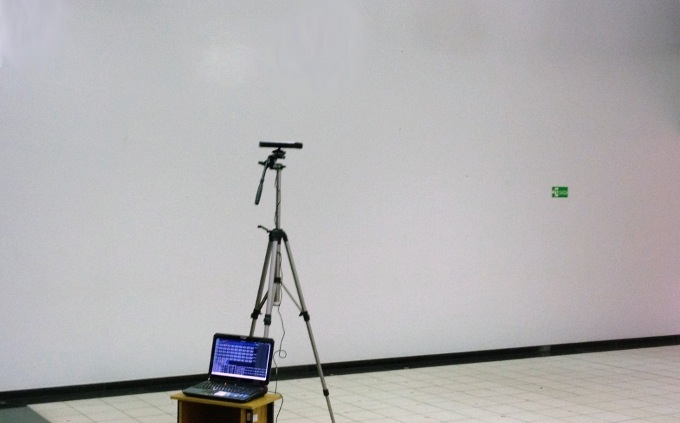
\includegraphics[width=.5\textwidth]{img/expSetup.jpg}} \qquad
%\subfigure[The blue dots show the spatial distribution of sensor \emph{poses}. Here we can see the sensor placed at one of the \emph{poses}]{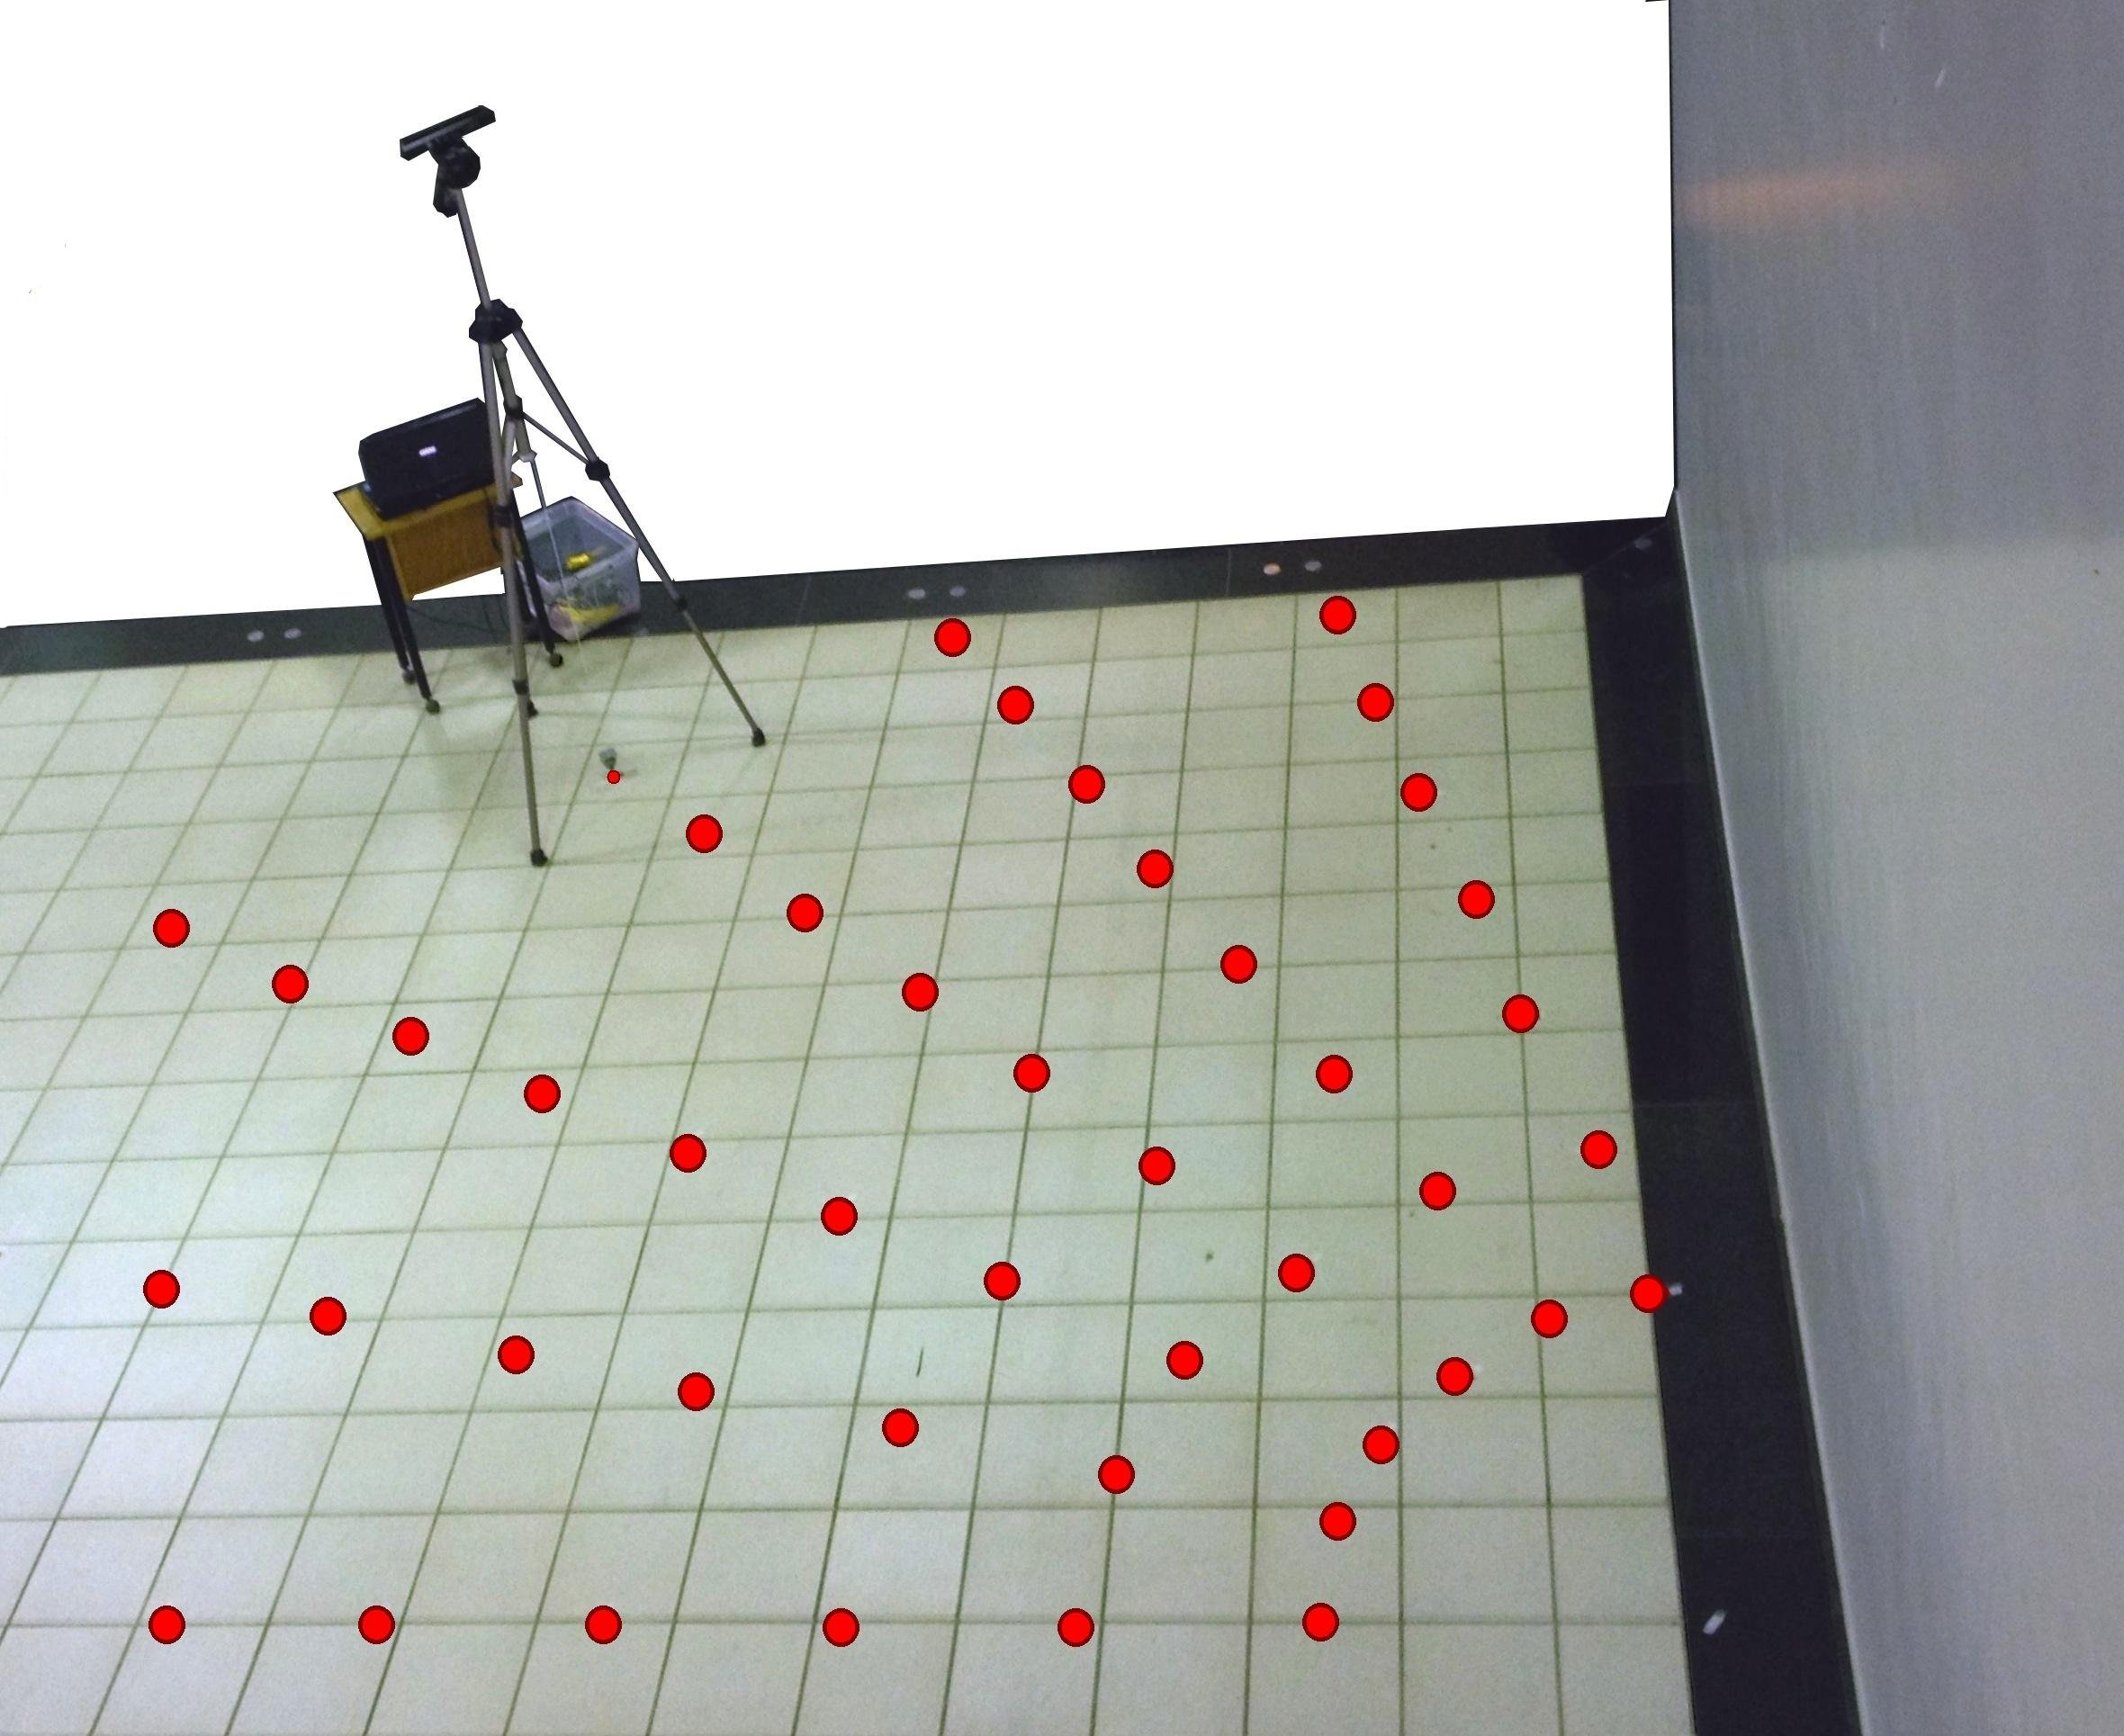
\includegraphics[width=.5\textwidth]{img/expSetup_markers.jpg}} \qquad
%\caption{The setup for obtaining our data set}
%\label{fig:exp_setup}
%\end{figure} 

%\begin{equation}
%%\scalebox{1}{$
%\begin{array}{lcc}
%	p_{hit}(z_t^k|x_t,m) = \eta \ \mathcal{N}\left(z_t^k;z_t^{k*},\sigma^2_{hit}\right) \text{; if} \ 0\leq z_t^k\leq z_{max} \\[.1cm]
%	\mathcal{N}\left(z_t^k;z_t^{k*},\sigma^2_{hit}\right) = \left(2\pi\sigma^2_{hit}\right)^{-1/2} \text{exp}\left(-\frac{1}{2}\frac{z_t^k-z_t^{k*}}{\sigma^2_{hit}}\right)
%\end{array}
%%$}
%\label{eq:mp} 
%\end{equation}
